\section{Auswertung}
\label{sec:Auswertung}

\subsection{Gegengekoppelter Verstärker}

Die Messwerte, die mit den vier verschiedenen Widerstandskombinationen aufgenommen wurden, sind in den Tabellen \ref{tab:gegen_kombi_1}, \ref{tab:gegen_kombi_2}, \ref{tab:gegen_kombi_3} und \ref{tab:gegen_kombi_4} eingetragen. Dort sind die Kombinationen einer Nummer zugeordnet mit der sie im folgenden bezeichnet werden.
Die Fehler werden wie folgt angenommen: $\Delta_\nu = \num{0.1} \nu, \sigma_U = \SI{10}{\milli\volt}$. Graphisch dargestellt sind die Messwerte sowie ein Fit an die Messwerte, die händisch der Flanke zugeordnet werden, in Abbildung \ref{fig:gegen} zu sehen. Außerdem wurden bei Notwendigkeit Werte dem Übergang zwischen Plateau und Flanke zugeordnet oder nicht berücksichtigt, wenn die Abweichung von den anderen Werten zu stark den Fit verfälscht hätte.
\begin{figure}
  \centering
  \includegraphics[width=1.2\textwidth]{build/gegen.pdf}
  \caption{Messwerte und Flankenfit aller vier Widerstandskombinationen.}
  \label{fig:gegen}
\end{figure}
Dieser Fit folgt der Gleichung:
\begin{align}
  \ln(V') = m \ln(\nu/\si{\kilo\hertz}) + b.
\end{align}
Dabei ergeben sich die Werte aus Tabelle \ref{tab:gegen_fits}. Außerdem ist in Tabelle \ref{tab:gegen_ergebnisse} der Mittelwert der Messwerte der Plateaus angegeben, sowie die prozentuale Abweichung von $V'_\text{Theorie}$. Dort ist auch die Grenzfrequenz eingetragen, die aus dem Schnittpunkt der gefitteten Graden mit der Linie auf Höhe von $V'_\text{Plateau}/\sqrt{2}$ beziehungsweise $V'_\text{Plateau}\cdot\sqrt{2}$ gewonnen wird.

%Fits
\begin{table}[h]
  \centering
  \begin{tabular}{S[table-format=1.0]
    S[table-format=2.3] @{${}\pm{}$} S[table-format=1.3]
    S[table-format=2.2] @{${}\pm{}$} S[table-format=1.2]}
    \toprule
    {i} & \multicolumn{2}{c}{$m$} & \multicolumn{2}{c}{$b$}\\
    \midrule
    1 & -0.841 & 0.006 & 4.55 & 0.04 \\
    2 & 0.29 & 0.03 & -3.6 & 0.2 \\
    3 & -0.74 & 0.08 & 4.2 & 0.5 \\
    4 & -0.87 & 0.04 & 4.7 & 0.2 \\
    \bottomrule
  \end{tabular}
  \caption{Ergebnisse aus der Messung mit gegengeschaltetem Operationsverstärker. Dabei ist $i$ die Nummer der Widerstandskombination; definiert in den Tabellen der Messwerte im Anhang.}
  \label{tab:gegen_fits}
\end{table}



Nun wird das Verstärkungs-Bandbreite-Produkt mit der Beziehung $VB = \nu'_\text{g} V'_\text{Plateau}=$ const überprüft. Es ergeben sich die Werte aus Tabelle \ref{tab:gegen_ergebnisse}. Da die zweite Kombination sich stark von den anderen unterscheidet, dadurch dass sie abschwächt und nicht verstärkt, wird sie zur Überprüfung der Konstanz nicht herangezogen.
Der Mittelwert aus den anderen Kombinationen beträgt:
\begin{align*}
  \frac{1}{3}\sum_{i=1, i\neq2}^4 \nu'_{\text{g}, \text{i}} V'_\text{i} = \SI{324(58)}{\kilo\hertz}.
\end{align*}

Außerdem wird für den gegengekoppelten Verstärker die endliche Leerlaufverstärkung $V$ mit
\begin{align}
  V = \left(\frac{1}{V'_\text{Plateau}} - \frac{R_1}{R_\text{N}}\right)^{-1}
\end{align}
nach Formel \eqref{eqn:leerlaufverst} abgeschätzt. Die Werte finden sich ebenfalls in Tabelle \ref{tab:gegen_ergebnisse}.
% \begin{align*}
%   V_1 = \num{-70(10)} \quad V_2 = \num{-3(5)} \quad V_3 = \num{32(26)} \quad V_4 = \num{300(500)}.
% \end{align*}

Zuletzt wird in Abbildung \ref{fig:phase} die Abhängigkeit der Phasendifferenz zwischen Eingangs- und Ausgangsspannung von der Frequenz dargestellt.

\begin{figure}
  \centering
  \includegraphics[width=0.9\textwidth]{build/phasen.pdf}
  \caption{Messwerte der Phasendifferenz zwischen Eingangs- und Ausgangsspannung aller vier Widerstandskombinationen.}
  \label{fig:phase}
\end{figure}

%Ergebnisse
\begin{table}[h]
  \centering
  \begin{tabular}{S[table-format=1.0]
    S[table-format=3.0]
    S[table-format=1.4] @{${}\pm{}$} S[table-format=1.4]
    S[table-format=1.0] @{${}\pm{}$} S[table-format=1.0]
    S[table-format=3.1] @{${}\pm{}$} S[table-format=1.1]
    S[table-format=3.0] @{${}\pm{}$} S[table-format=3.0]}
    \toprule
    {i} & {$\nu'_\text{g}\:/\:\si{\kilo\hertz}$} & \multicolumn{2}{c}{$\bar V'_\text{Plateau}$} &
    \multicolumn{2}{c}{$\Delta_{V'}\:/\:\si{\percent}$} & \multicolumn{2}{c}{$VB\:/\:\si{\kilo\hertz}$}& \multicolumn{2}{c}{$V$}\\
    \midrule
    1 & 334 & 1.001 & 0.02 & 1 & 3 & 338 & 8 & -70 & 10\\
    2 & 369 & 0.1038 & 0.0004 & 3 & 5 & 38.2 & 0.1 & -3 & 5\\
    3 & 193 & 2.00 & 0.02 & 6 & 5 & 386 & 4 & 32 & 26\\
    4 & 25 & 9.6 & 0.2 & 3 & 5 & 247 & 4 & 300 & 500\\
    \bottomrule
  \end{tabular}
  \caption{Ergebnisse aus der Messung mit gegengeschaltetem Operationsverstärker. Dabei ist $i$ die Nummer der Widerstandskombination; definiert in den Tabellen der Messwerte im Anhang.}
  \label{tab:gegen_ergebnisse}
\end{table}

\subsection{Umkehr-Integrator und -Differentiator}

\paragraph{Umkehr-Integrator}

Zunächst werden auf die Schaltung des Umkehr-Integrators drei verschiedene Eingangsspannung gegeben.
In der Schaltung werden für Widerstand und Kondensator Bauteile mit folgenden  Werten verwendet:
\begin{align*}
  R = \SI{99.7(5)}{\kilo\ohm} \quad C = \SI{970(10)}{\nano\farad}.
\end{align*}
Der Verlauf der Ausgangsspannung sowie der Eingangsspannung sind in den Abbildungen \ref{fig:int_recht}, \ref{fig:int_drei} und \ref{fig:int_sin} zu sehen. Dabei ist die Eingangsspannung in orange und die Ausgangsspannung in grün abgebildet. In Abbildung \ref{fig:int_recht} ist die Eingangsspannung eine Rechteckspannung und der Integrator integriert den die konstanten Spannungsplateaus dieser auf, sodass die Ausgangsspannung als Dreieckspannung zu erkennen ist. Im nächsten Bild wird eine Dreieckspannung integriert. Da dort die Spannung eine Anstiegszeit besitzt, nimmt die Spannung des Integrals erst langsam zu, wird dann steiler und nimmt wieder ab, wenn die Spannung des Dreieckssignals den Scheitelpunkt erreicht hat. Das Ergebnis ist eine Sinusspannung. Beim hier letzten Bild geht eine Sinusspannung ein und der Integrator liefert aus gleichen Gründen wie oben auch eine Sinusspannung.

\begin{figure}
  \centering
  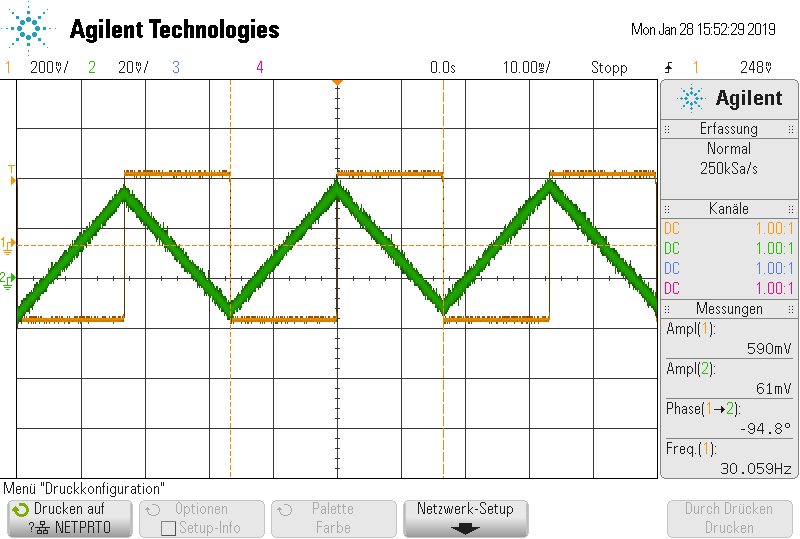
\includegraphics[width=0.8\textwidth]{Schlager/scope_16.png}
  \caption{Das Oszilloskopbild des Umkehr-Integrators bei angelegter Rechteckspannung.}
  \label{fig:int_recht}
\end{figure}
\begin{figure}
  \centering
  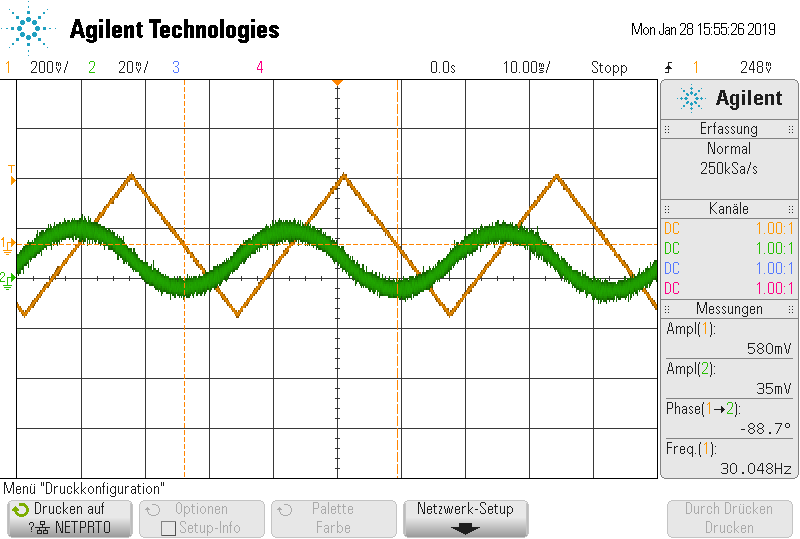
\includegraphics[width=0.8\textwidth]{Schlager/scope_17.png}
  \caption{Das Oszilloskopbild des Umkehr-Integrators bei angelegter Dreiecksspannung.}
  \label{fig:int_drei}
\end{figure}
\begin{figure}
  \centering
  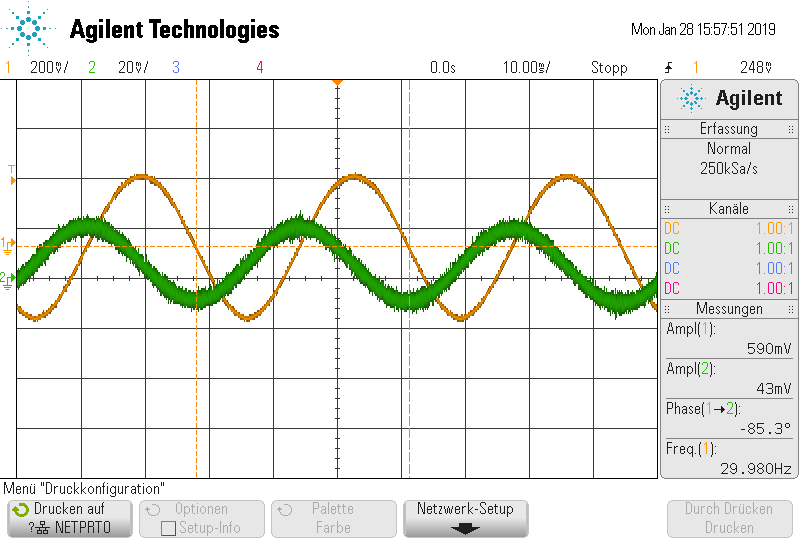
\includegraphics[width=0.8\textwidth]{Schlager/scope_18.png}
  \caption{Das Oszilloskopbild des Umkehr-Integrators bei angelegter Sinusspannung.}
  \label{fig:int_sin}
\end{figure}

Außerdem wird die Verstärkung $V' = U_\text{A}/U_0$ gegen die Kreisfrequenz $\omega$ aufgetragen. Dabei ist die Eingangsspannung sinusförmig. Die Messwerte sind in Tabelle \ref{tab:int_werte} zu finden. Zum Fitten und Abbilden werden jetzt allerdings die Werte logarithmiert. Damit ergibt sich als Fitfunktion nach Formel \eqref{eqn:int_aus}:
\begin{align}
  \begin{split}
  \ln(V') &= \ln\left((k\omega)^m\right)\\
          &= m \ln(\omega) + m \ln(k)\\
          &= m \ln(\omega) + b
    \end{split}
\end{align}
Aus dem Fit, der zusammen mit den Messwerten in Abbildung \ref{fig:int_fit} zu sehen ist, folgt:
\begin{align*}
  m &= \num{-0.86(7)}\\
  b &= (\num{2.1(4)})\: \ln(\Omega \text{F}).
\intertext{Damit ist}
k &= \exp\left(\frac{b}{m}\right) = \SI{0.09(4)}{\ohm\farad}
\intertext{Die prozentuale Abweichung von dem nach Formel \eqref{eqn:int_aus} erwarteten Wert beträgt:}
  \Delta_{k, RC} &= \SI{10(40)}{\percent}.
\end{align*}

\begin{figure}
  \centering
  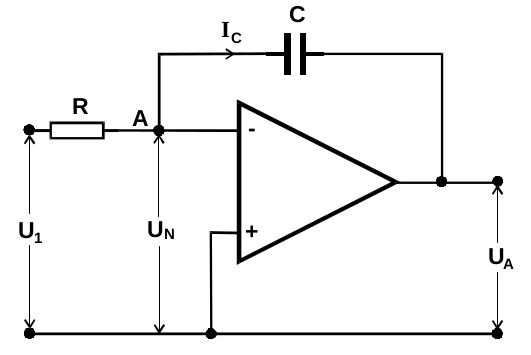
\includegraphics[width=0.8\textwidth]{build/integrator.pdf}
  \caption{Die frequenzabhängige Verstärkung des Umkehr-Integrators bei angelegter Sinusspannung.}
  \label{fig:int_fit}
\end{figure}

\paragraph{Umkehr-Differentiator}

Zunächst werden auf die Schaltung des Umkehr-Differentiators drei verschiedene Eingangsspannung gegeben.
In der Schaltung werden für Widerstand und Kondensator Bauteile mit folgenden  Werten verwendet:
\begin{align*}
  R = \SI{1.00(5)}{\kilo\ohm} \quad C = \SI{970(10)}{\nano\farad}.
\end{align*}
Der Verlauf der Ausgangsspannung sowie der Eingangsspannung sind in den Abbildungen \ref{fig:diff_recht}, \ref{fig:diff_drei} und \ref{fig:diff_sin} zu sehen. Dabei ist die Eingangsspannung in orange und die Ausgangsspannung in grün abgebildet. In Abbildung \ref{fig:diff_recht} wird eine Rechteckspannung auf die Schaltung gegeben. Der Differentiator liefert dann an den Stellen maximaler Steigung Delta-Peak-ähnliche Ausschläge. Dies ist verständlich, da er das Eingangssignal ableitet. So wird im nächsten Bild eine Dreieckspannung in eine Rechteckspannung überführt, da sie eine konstante Steigung besitzt, dessen Vorzeichen wechselt. In Abbildung \ref{fig:diff_sin} wird eine eingehende Sinusspannung abgeleitet zu einer Cosinusspannung genau wie erwartet.

\begin{figure}
  \centering
  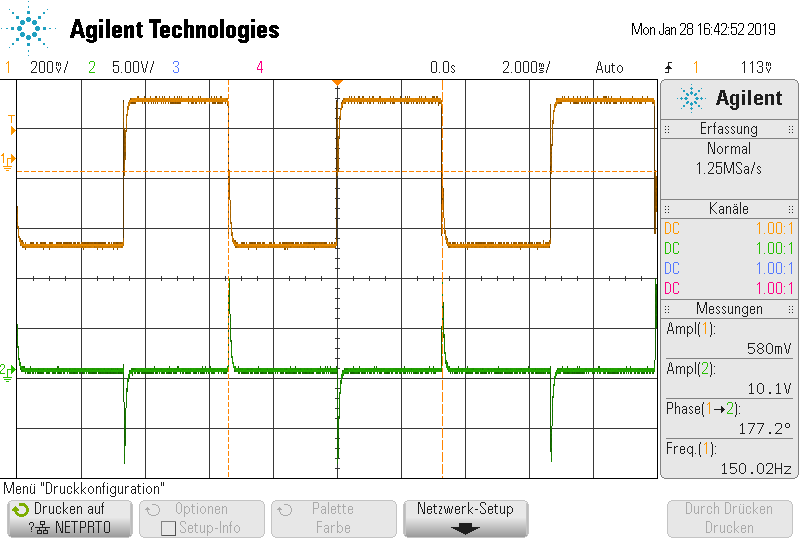
\includegraphics[width=0.8\textwidth]{Schlager/scope_20.png}
  \caption{Das Oszilloskopbild des Umkehr-Differentiators bei angelegter Rechteckspannung.}
  \label{fig:diff_recht}
\end{figure}
\begin{figure}
  \centering
  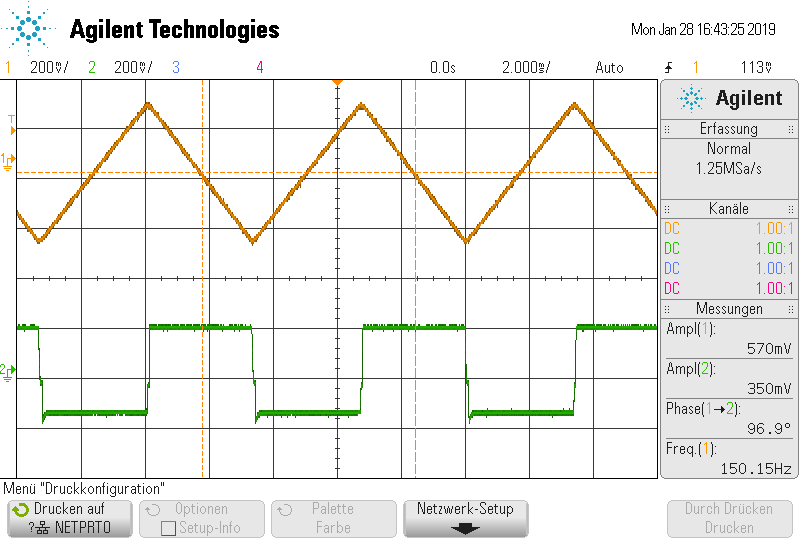
\includegraphics[width=0.8\textwidth]{Schlager/scope_21.png}
  \caption{Das Oszilloskopbild des Umkehr-Differentiators bei angelegter Dreiecksspannung.}
  \label{fig:diff_drei}
\end{figure}
\begin{figure}
  \centering
  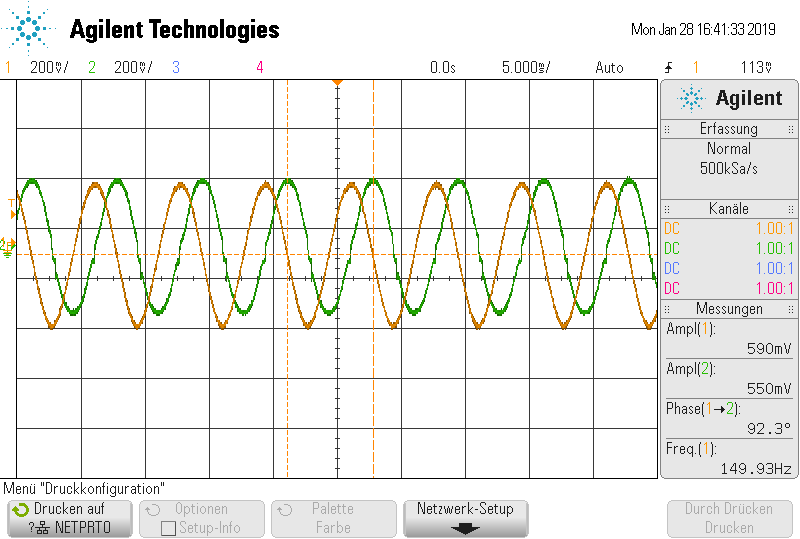
\includegraphics[width=0.8\textwidth]{Schlager/scope_19.png}
  \caption{Das Oszilloskopbild des Umkehr-Differentiators bei angelegter Sinusspannung.}
  \label{fig:diff_sin}
\end{figure}

Außerdem wird die Verstärkung $V' = U_\text{A}/U_0$ gegen die Kreisfrequenz $\omega$ aufgetragen. Dabei ist die Eingangsspannung sinusförmig. Die Messwerte sind in Tabelle \ref{tab:diff_werte} zu finden.
Die Fitfunktion nach Formel \eqref{eqn:diff_aus} lautet:
\begin{align}
  V' = k \omega.
\end{align}
Aus dem Fit, der zusammen mit den Messwerten in Abbildung \ref{fig:diff_fit} zu sehen ist, folgt:
\begin{align*}
  k = \SI{9.64(5)e-4}{\ohm\farad}.
\intertext{Die prozentuale Abweichung von dem nach Formel \eqref{eqn:diff_aus} erwarteten Wert beträgt:}
  \Delta_{k, RC} = \SI{1(5)}{\percent}.
\end{align*}

\begin{figure}
  \centering
  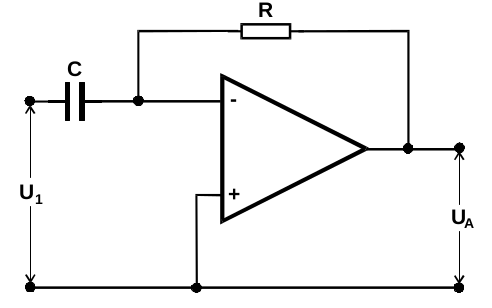
\includegraphics[width=0.8\textwidth]{build/differentiator.pdf}
  \caption{Die frequenzabhängige Verstärkung des Umkehr-Differentiators bei angelegter Sinusspannung.}
  \label{fig:diff_fit}
\end{figure}

\subsection{Schmitt-Trigger}

Die Schaltung nach Abbildung \ref{fig:schmitttrigger} liefert das Oszilloskopbild aus Abbildung \ref{fig:schmitt}.
\begin{figure}
  \centering
  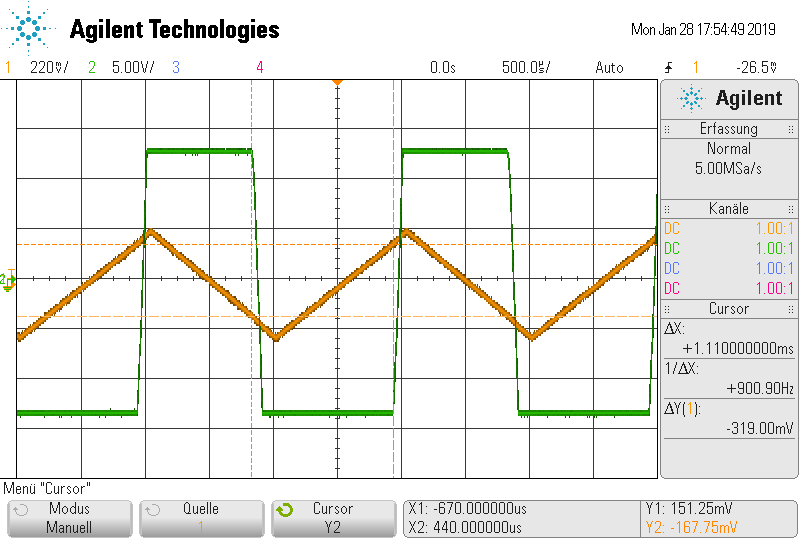
\includegraphics[width=0.8\textwidth]{Schlager/scope_22.png}
  \caption{Das Oszilloskopbild des Schmitt-Triggers mit den Spannungsmesswerten an den Stellen, an denen die Ausgangsspannung umschlägt. Hier ist die Eingangsspannung in orange und die Ausgangsspannung in grün zu sehen.}
  \label{fig:schmitt}
\end{figure}
Der Wert der eingebauten Widerstände beträgt:
\begin{align*}
  R_1 &= \SI{1.00(5)}{\kilo\ohm} \quad R_\text{p} = \SI{99.7(5)}{\kilo\ohm}
  \intertext{Die Betriebsspannung beträgt:}
  U_\text{B} &= \SI{14.13(5)}{\volt}.
\end{align*}
Die aus Abbildung \ref{fig:schmitt} abgelesenen Werte für die Schwellenspannung sind:
\begin{align*}
  U_\text{e, Schwelle, 1} &= \SI{151(5)}{\milli\volt} \quad U_\text{e, Schwelle, 2} = \SI{-168(5)}{\milli\volt}.
\intertext{Die Abweichung von dem erwarteten Wert $R_1/R_\text{p} U_\text{B}$ betragen:}
  \Delta_{1} &= \SI{7(6)}{\percent} \quad \Delta_{2} = \SI{18(7)}{\percent}.
\end{align*}

Außerdem kann in Abbildung \ref{fig:schmitt2} noch die Amplitude der Ausgangsspannung abgelesen werden. Ihr Wert und die Abweichung vom erwarteten Wert $2 U_\text{B}$ betragen:
\begin{align*}
  U_\text{A} = \SI{26.3(5)}{\volt} \quad \Delta_{U_\text{A}} = \SI{7(2)}{\percent}.
\end{align*}

\subsection{Signalgenerator}

Die Schaltung nach Abbildung \ref{fig:signalgen} liefert das Oszilloskopbild aus Abbildung \ref{fig:signalgenoszi}.
\begin{figure}
  \centering
  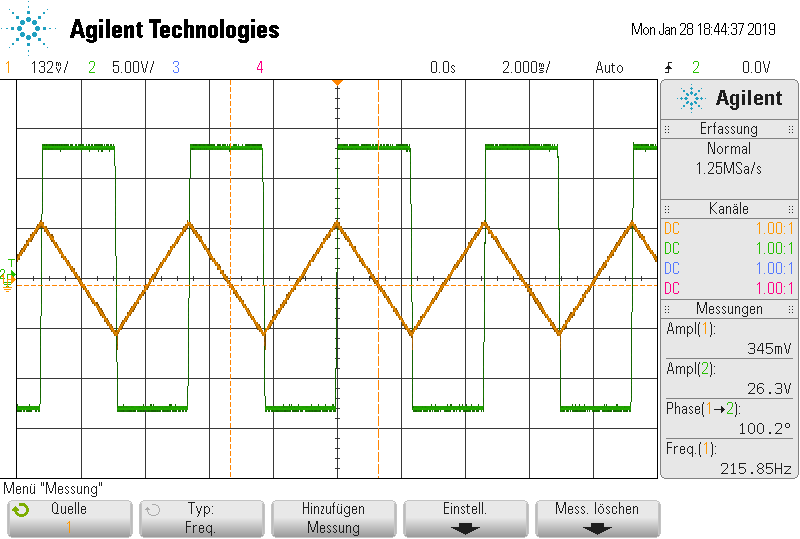
\includegraphics[width=0.8\textwidth]{Schlager/scope_25.png}
  \caption{Das Oszilloskopbild des Signalgenerators mit der generierten Dreieck- und Rechteckspannung.}
  \label{fig:signalgenoszi}
\end{figure}
Dabei haben die Bauteile folgende Werte:
\begin{align*}
  R_1 &= \SI{1.00(5)}{\kilo\ohm} \quad R_\text{p} = \SI{99.7(5)}{\kilo\ohm}\\
  R &= \SI{100.0(5)}{\kilo\ohm}\quad C = \SI{970(10)}{\nano\farad}.
\end{align*}

Die Amplituden der beiden Spannungen, sowie die Frequenz können nun mit den berechneten Werten verglichen werden.
Die gemessenen Werte sind:
\begin{align*}
  U_\text{Dreieck} = \SI{345(5)}{\milli\volt} \quad U_\text{Rechteck} = \SI{26.3(5)}{\volt} \quad \omega = \SI{1.357(6)}{\kilo\hertz}
\end{align*}
Zur Berechnung der erwarteten Dreiecksspannung wird Formel \eqref{eqn:ampl_drei} und für die Frequenz Formel \eqref{eqn:freq_signalgen} \todo{richtige Formel benutzen} genutzt. Der erwartete Wert der Rechteckspannung beträgt erneut $2 U_\text{B}$.
Die erwarteten Werte sind also:
\begin{align*}
  U_\text{Dreieck, erw.} &= \SI{284(14)}{\milli\volt} \quad U_\text{Rechteck, erw.} = \SI{28.25(10)}{\volt} \quad \omega_\text{erw.} = \SI{3.22(17)}{\kilo\hertz}
\intertext{Die Abweichung beträgt dann:}
 \Delta_\text{$U_\text{Dreieck}$} &= \SI{22(6)}{\percent} \quad \Delta_\text{$U_\text{Rechteck}$} = \SI{7(2)}{\percent} \quad \Delta_{\omega} = \SI{58(2)}{\percent}.
\end{align*}

\subsection{Entdämpfte und Gedämpfte Schwingung}

\paragraph{Entdämpfte Schwingung}

\begin{figure}
  \centering
  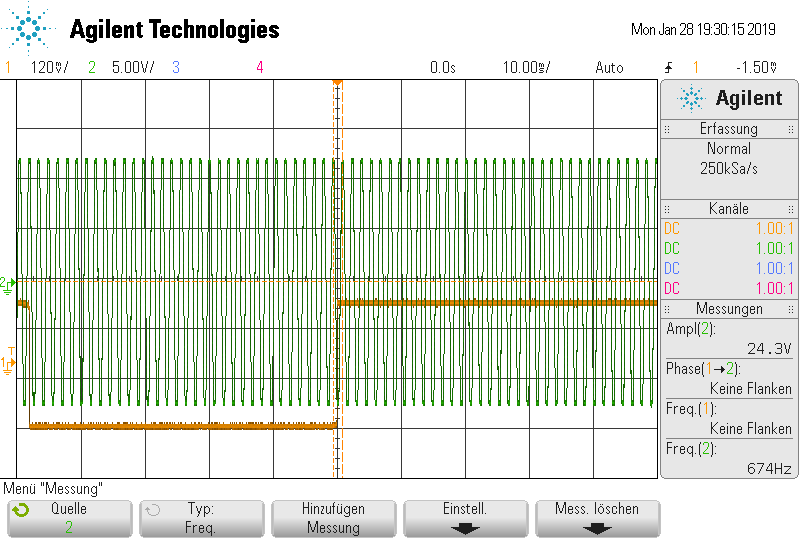
\includegraphics[width=0.8\textwidth]{Schlager/scope_28.png}
  \caption{Das Oszilloskopbild der entdämpften Schwingung.}
  \label{fig:entdaempft}
\end{figure}
In Abbildung \ref{fig:entdaempft} ist das Oszilloskopbild der entdämpften Schwingung zu sehen.
Für den Widerstand $R$ und den Kondensator $C$ werden folgende Werte gemessen. Da zwei leicht verschiedene Kondensatoren benutzt werden (siehe Messwerte im Anhang), wird für den Wert $C$ der Mittelwert aus beiden angenommen:
\begin{align*}
  R = \SI{9.96(5)}{\kilo\ohm} \quad C = \SI{22(1)}{\nano\farad}.
\end{align*}
Die gemessene Frequenz beträgt:
\begin{align*}
  \nu_\text{gem.} = \SI{674(5)}{\hertz}.
\intertext{Nach Formel \eqref{eqn:freqexp} ist die erwartete Frequenz:}
  \nu_\text{erw.} = \SI{740(40)}{\hertz}.
\intertext{Die Abweichung beträgt:}
  \Delta_\nu = \SI{8(5)}{\percent}.
\end{align*}

\paragraph{Gedämpfte Schwingung}

\begin{figure}
  \centering
  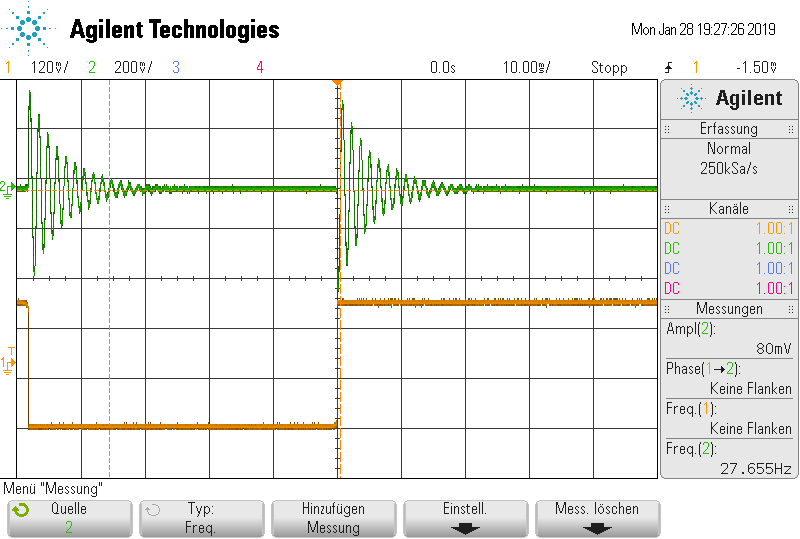
\includegraphics[width=0.8\textwidth]{Schlager/scope_26.png}
  \caption{Das Oszilloskopbild der gedämpften Schwingung.}
  \label{fig:gedaempft}
\end{figure}
In Abbildung \ref{fig:gedaempft} ist das Oszilloskopbild der gedämpften Schwingung zu sehen.
Die Werte für den Widerstand $R$ und den Kondensator $C$ sind dieselben wie im Kapitel zuvor.
An die Maximawerte einer abschwingenden Schwingung wird nun folgende Formel gefittet:
\begin{align}
  U_\text{A} = U_0 \text{e}^{- \frac{t}{\tau}}.
\end{align}
In Abbildung \ref{fig:gedaempft_fit} sind die Messwerte sowie der Fit zu sehen.
\begin{figure}
  \centering
  \includegraphics[width=0.8\textwidth]{build/gedaempft.pdf}
  \caption{Die Messwerte der gedämpften Schwingung sowie der Fit an die Maxima der Schwingung.}
  \label{fig:gedaempft_fit}
\end{figure}
Die Werte aus dem Fit sind:
\begin{align*}
  \tau &= \SI{4.78(6)}{\per\second} \quad U_0 = \SI{1.7(2)e-5}{\volt}
% \intertext{Der für $k$ erwartete Wert nach Formel \eqref{eqn:???} sowie die Abweichung des gemessenen davon betragen:}
%   20 R C &= \SI{4.4(3)e-3}{\ohm\farad} \quad \Delta_{k} = \SI{9(8)}{\percent}.
\end{align*}
\begin{align*}
  \intertext{Der für $\tau$ erwartete Wert nach Formel \eqref{eqn:tauentdämpft} sowie die Abweichung des gemessenen davon betragen:}
  20 R C &= \SI{4.4(3)}{\milli\second} \quad \Delta_{\tau} = \SI{9(8)}{\percent}.
\end{align*}





% \begin{figure}
%   \centering
%   \includegraphics{build/plotElement.pdf}
%   \caption{Plot.}
%   \label{fig:plot}
% \end{figure}
%
% Tabelle für copy and paste:
% \begin{table}[h]
%   \centering
%   \begin{tabular}{S S}
%     \toprule
%     {$k$} & {$U\:/\:\si{\milli\volt}$}\\
%     \midrule
%     1 & 637.2\\
%     3 & 212.4\\
%     5 & 127.4\\
%     7 & 91.03\\
%     9 & 70.8\\
%     \bottomrule
%   \end{tabular}
%   \caption{Amplituden Rechteckspannung.}
%   \label{tab:rechtampl}
% \end{table}
